\documentclass[border=3pt,tikz]{standalone}
\let\oldvec\vec
\usepackage{amsmath} % for \text
\usepackage{tikz}
\usetikzlibrary{decorations.pathreplacing,decorations.markings}
\usepackage{pgfplots}
\pgfplotsset{compat=1.14} 
\usepackage{comment}
\tikzset{>=latex} % for LaTeX arrow head
\usepackage{xcolor}

\providecommand{\sin}{} \renewcommand{\sin}{\hspace{2pt}\mathrm{sen}}
\usetikzlibrary{arrows}

\usetikzlibrary{decorations.markings,arrows.meta}
\tikzset{
      myarrowtip/.tip={Straight Barb[length=4pt,width=6pt]},
      setas histerese crescente/.style={%
      decoration={%
         markings,
         mark=at position 0.25 with \arrow{myarrowtip},
         mark=at position 0.5 with \arrow{myarrowtip},
         mark=at position 0.7 with \arrow{myarrowtip},
         },
         postaction=decorate}
      }%

\tikzset{
      myarrowtip/.tip={Straight Barb[length=4pt,width=6pt]},
      setas histerese decrescente/.style={
      decoration={
         markings,
         mark=at position 0.25 with \arrowreversed{myarrowtip},
         mark=at position 0.5 with \arrowreversed{myarrowtip},
         mark=at position 0.7 with \arrowreversed{myarrowtip},
         },
         postaction=decorate}
      }

\tikzset{
      myarrowtip/.tip={Straight Barb[length=4pt,width=6pt]},
      setas histerese inicial/.style={
      decoration={
         markings,
         mark=at position 0.5 with \arrow{myarrowtip},
         },
         postaction=decorate}
      }

\begin{document}

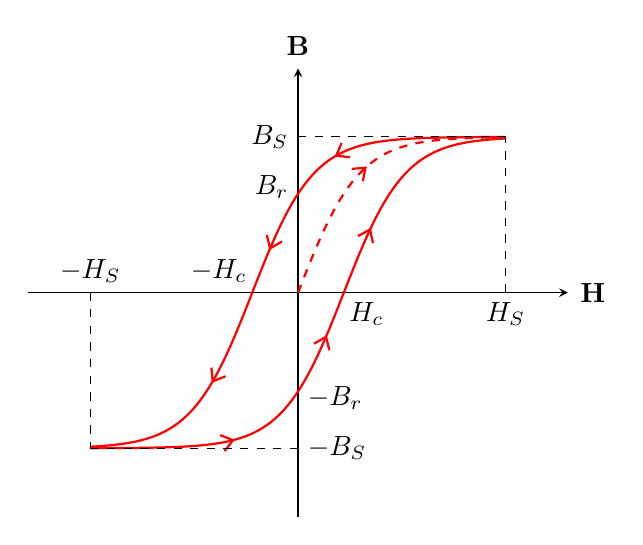
\begin{tikzpicture}

  \def\xlim{4}
  \def\ylim{4}
  \def\xaxis{\xlim*1.3}
  \def\yaxis{\ylim*0.9}
  
\begin{axis}[
                xmin=-\xaxis, xmax=\xaxis,
                ymin=-\yaxis, ymax=\yaxis,
                axis lines = middle,
                ticks=none,
                xlabel = {$\mathbf{H}$},
                ylabel = {$\mathbf{B}$},
                every axis x label/.style={at={(current axis.east)},right=1},
                every axis y label/.style={at={(current axis.north)},above=1},
            ]
\addplot [
            domain=-\xlim:\xlim, 
            samples=100, 
            color=red,
            thick,
            setas histerese crescente
         ]
        {5/(1 + exp(-1.7*x + 1.5)) - 2.5};

\addplot [
            domain=-\xlim:\xlim, 
            samples=100, 
            color=red,
            thick,
            setas histerese decrescente
         ]
        {5/(1 + exp(-1.7*x - 1.5)) - 2.5};

\addplot [
            domain=-0:\xlim, 
            samples=100, 
            color=red,
            thick,
            dashed,
            setas histerese inicial
         ]
        {5/(1 + exp(-1.7*x)) - 2.5};

\draw [dashed] (4,0) node[below] {$H_S$} -- (4,2.5);
\draw [dashed] (0,2.5) node[left] {$B_S$} -- (4,2.5);
\draw [dashed] (-4,0) node[above] {$-H_S$} -- (-4,-2.5);
\draw [dashed] (0,-2.5) node[right] {$-B_S$} -- (-4,-2.5);
\draw (0,1.7) node[left] {$B_r$};
\draw (0,-1.7) node[right] {$-B_r$};
\draw (-0.8,0) node[above left] {$-H_c$};
\draw (0.8,0) node[below right] {$H_c$};

\end{axis}



\end{tikzpicture}

\end{document}